\subsection{Introducción}
Con certeza, es posible afirmar que la onda senoidal es una de las formas de onda fundamentales tanto en el sentido matemático, puesto que cualquier otra forma de onda se puede expresar como una combinación de Fourier de ondas senoidales básicas, como en el
sentido práctico, debido a que se usa en forma extensiva como señal de prueba, de referencia
y como portadora. A pesar de su simplicidad, su generación resulta una tarea demandante si
se desea estar cerca de la pureza. Asimismo, los circuitos de amplificadores operacionales que han obtenido
mayor prominencia en la generación de ondas senoidales son el oscilador de puente de Wien
y el oscilador de cuadratura, de los cuales a continuación se expondrá únicamente el oscialdor de Wien.

\subsection{Oscilador Básico de puente de Wien.}
En el circuito de la Figura (\ref{fig:wienbasico}) se emplea tanto retroalimentación negativa, a través de $R_2$ y $R_1$, como retroalimentación positiva, a través de los circuitos RC en serie y en paralelo. Además, el comportamiento del circuito resulta afectado por la prevalencia de dichas retroalimentaciones. Es necesario que los componentes de los circuitos RC no tengan los mismos valores. Sin embargo, si éstos se igualan, se simplifica el análisis. En la Figura (\ref{fig:wienbasico1}) se puede ver como la configuración no inversora amplifica a $V_p$ en la cantidad dada por la siguiente ecuación:
\begin{align}
	A=\frac{V_0}{V_p}=1+\frac{R_2}{R_1}
\end{align}

\begin{figure}[H]
\centering
\begin{subfigure}{.49\textwidth}
\centering
	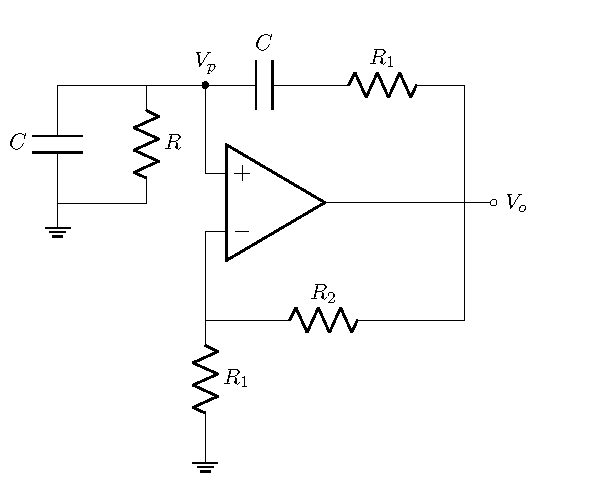
\includegraphics[width=\textwidth, page=1]{Imagenes-Ej1/Circuitos1.pdf}
	\caption{Circuito del puente.}
	\label{fig:wienbasico1}
\end{subfigure}
\begin{subfigure}{.49\textwidth}
\centering
	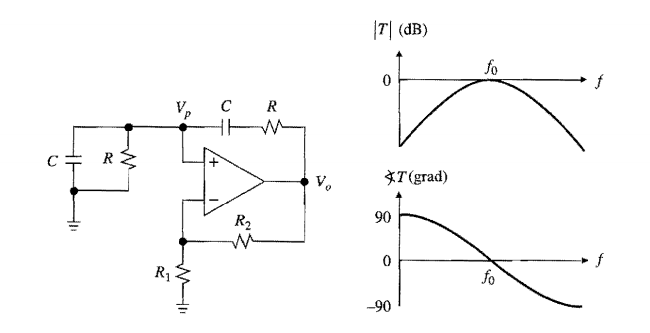
\includegraphics[width=0.7\textwidth,trim={9.5cm 0 0 0},clip]{Imagenes-Ej1/102.png}
	\caption{Lazo de ganancia T(jf) para el caso $\frac{R_2}{R_1} =2$. }
	\label{fig:wienbasico2}
\end{subfigure}
\caption{Oscilador de Wien.}
\label{fig:wienbasico}
\end{figure}

Por simplicidad, se supone un amplificador operacional ideal en el circuito presentado. Luego, se sustituye $V_p$ por el mismo amplificador operacional a través de los dos circuitos RC como:
\begin{align}
V_p= V_o \frac{Z_p}{Z_p+Z_s}
\end{align}
\begin{equation}
\begin{split}
	Z_p = & R // \frac{1}{j2\pi f C} \\
	Z_s = & R + \frac{1}{j2\pi f C} 
\end{split}
\end{equation}

A partir de estas expresiones se puede despejar.
\begin{align}
\beta (jf)=\frac{V_p}{V_o}=\frac{1}{3+j\cdot \left( \frac{f}{f_0}-\frac{f_0}{f} \right) }
\end{align}

Donde $f_o = \frac{1}{2\pi RC}$. La ganancia total experimentada por una señal al recorrer el lazo es
$T(jf)=A \cdot B$.
\begin{align}
T (jf)=\frac{1+\frac{R_2}{R_1}}{3+j\cdot \left( \frac{f}{f_0}-\frac{f_0}{f} \right) }
\end{align}

Esta es una función pasa banda, puesto que se aproxima a cero tanto en frecuencias altas como en bajas. Su valor pico ocurre en $f= fo$, siendo igual a
\begin{align}
	T (jf)=\frac{1+\frac{R_2}{R_1}}{3}
\label{eq:107}
\end{align}

El hecho de que $T(jf_o)$ sea real indica que una señal de frecuencia $f_o$ experimenta un cambio de fase neto de cero al recorrer el lazo. Dependiendo de la magnitud de $T(jf_o)$, existen tres posibilidades distintas: 
\begin{enumerate}
\item  	$T(jf_o) < 1$, esto es, $A < 3 $. Cualquier perturbación de frecuencia $f_o$ surgida en la
entrada del amplificador operacional, primero es amplificada por $A < 3$, y después por $B(jf_o) =\frac{1}{3}$, para una ganancia neta menor de uno. La intuición indica que esta perturbación se reduce cada vez que recorre el lazo hasta que de manera eventual decae hasta cero. Así, es posible establecer que la retroalimentación negativa (a través de R2 y R1) prevalece sobre la retroalimentación positiva (a través de Zs y Zp), lo que resulta en un sistema estable. En consecuencia, los polos del circuito descansan en la mitad izquierda del plano complejo. 
\begin{figure}[H]
	\centering
	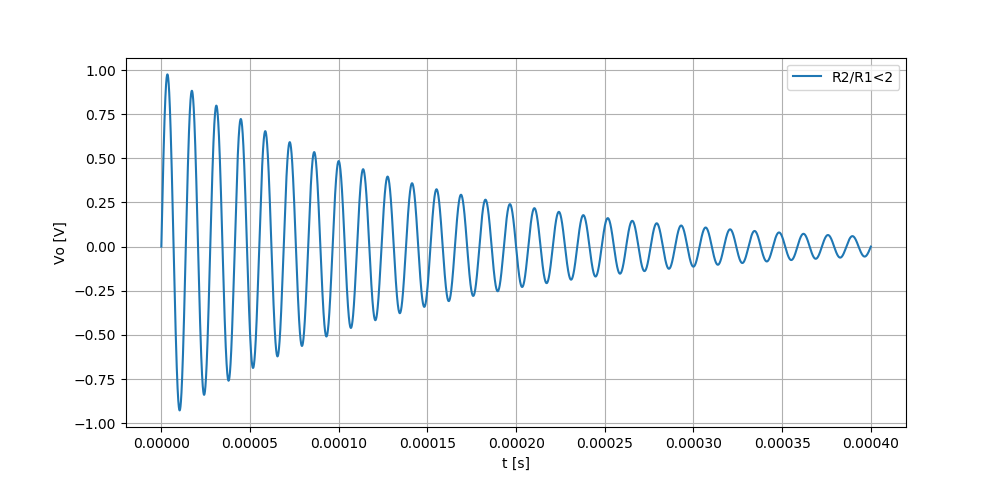
\includegraphics[width=\textwidth]{Imagenes-Ej1/r1r2m.png}
	\label{fig:r1r2m}
	\caption{$V_0 \implies \frac{R_2}{R_1}<2$}
\end{figure}
\item 	 $T(jf_o) > 1$, esto es, $A> 3$. Ahora la retroalimentación positiva prevalece sobre la
negativa, lo cual indica que una perturbación de frecuencia $f_o$ se amplificará en forma regenerativa, ocasionando que el circuito rompa en oscilaciones de magnitud creciente. Así, el circuito es inestable y sus polos se encuentran en la mitad derecha del plano complejo. Como es sabido, las oscilaciones se presentan hasta que se alcancen los límites de saturación del amplificador operacional. Después de eso, cuando se observe a $V_o$ con el osciloscopio, aparece como una onda senoidal recortada.
\begin{figure}[H]
	\centering
	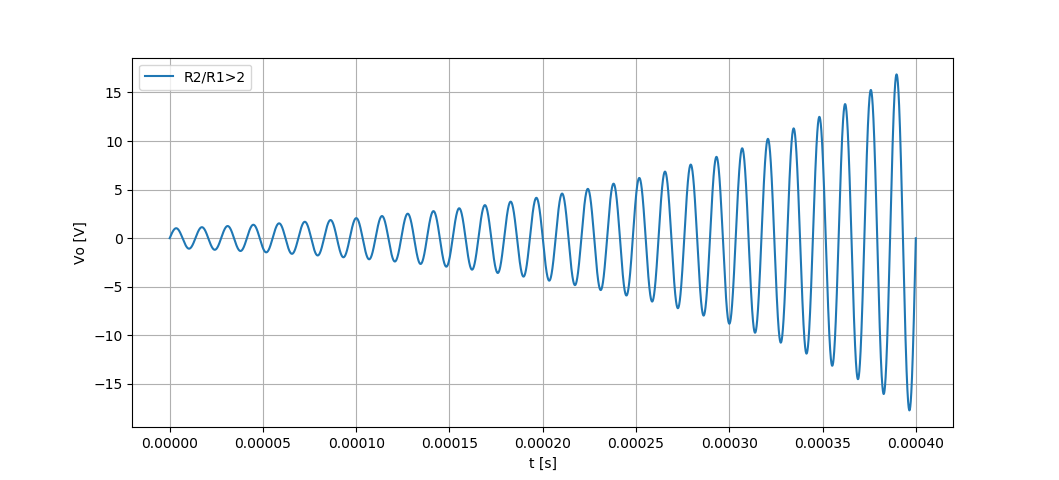
\includegraphics[width=\textwidth]{Imagenes-Ej1/r1r2g.png}
	\label{fig:r1r2g}
	\caption{$V_0 \implies \frac{R_2}{R_1}>2$}
\end{figure}
\item  $T(jf_o) = 1$, o bien $A= 3$. Esta condición se denomina como estabilidad neutral, debido a que las retroalimentaciones se aplican en cantidades iguales. Cualquier perturbación de frecuencia $f_o$ primero es amplificada por 3 y luego por $\frac{1}{3}$, lo cual indica que, una vez iniciada, se sostiene en forma indefinida. Como es sabido, esto corresponde a un par de polo que está justo sobre el eje $j \omega$. Las condiciones $\sphericalangle T(jf_0)= 0^\circ$ y $|T(jfo)|= 1$, en conjunto se denominan como el criterio de Barkhausen, para la oscilación en $f=f_o$. La naturaleza pasa banda de $T(jf)$ permite que la oscilación ocurra sola. Además, cualquier intento de oscilación en otras frecuencias se desalienta en forma natural, debido a que ahí $\sphericalangle T(jf_0) \neq 0^\circ$ y $|T(jf)| < 1$. Con base a lo expresado en (\ref{eq:107}), la estabilidad neutral se alcanza con 
\begin{align}
\frac{R_2}{R_1}=2
\end{align}

Resulta evidente que, cuando se cumple esta condición, los componentes alrededor del amplificador operacional forman un puente balanceado en $f=f_o$.
\begin{figure}[H]
	\centering
	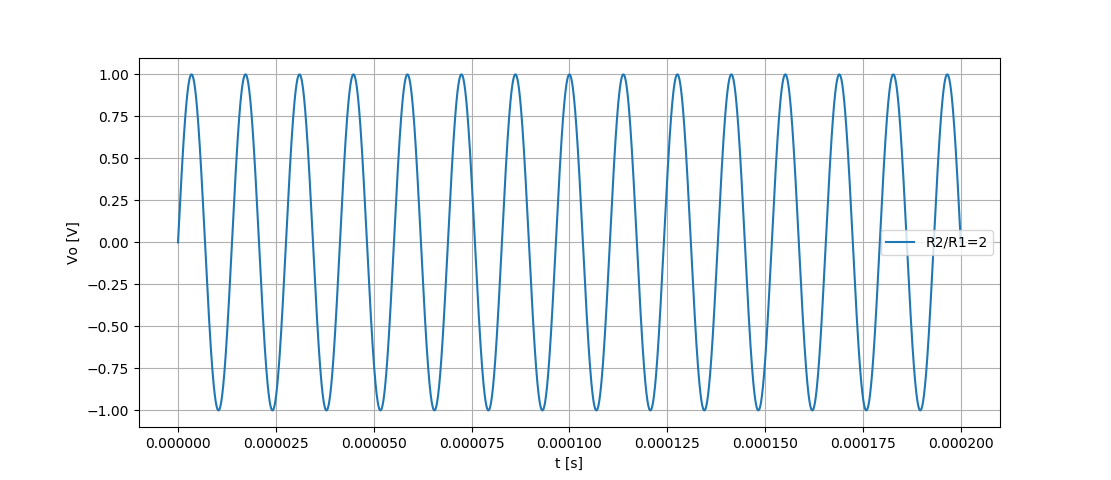
\includegraphics[width=\textwidth]{Imagenes-Ej1/r2r1e.png}
	\label{fig:r1r2e}
	\caption{$V_0 \implies \frac{R_2}{R_1}=2$}
\end{figure}
\end{enumerate}

Finalmente se obtiene la transferencia del circuito:
\begin{align}
H(s)=\frac{T(s)}{1-T(s)}\cdot \frac{1}{\beta}
\end{align}

En papel, la condición de equilibrio se da sin ningún problema. Por otro lado, en un circuito implementado en la realidad, la dispersión de los componentes hace difícil mantener al puente balanceado de manera exacta. Además, se deben tomar ciertas precauciones, como lo son: 
\begin{itemize}
\item El inicio en forma espontánea al encender el circuito.
\item El hecho de que amplitud se debe mantener por debajo de los límites de saturación del amplificador operacional, así se evita la distorsión excesiva.
\end{itemize}

Estos objetivos se satisfacen haciendo que la relación $\frac{R_2}{R_1}$ sea dependiente de la
amplitud, de manera que en los niveles bajos de señal esta sea sólo un poco mayor que 2
para asegurar que la oscilación inicie, mientras que en los altos sea sólo un poco
menor que 2 para limitar la amplitud. Entonces, una vez que la oscilación ha iniciado, esta
crece y se estabiliza de forma automática en algún nivel intermedio donde $\frac{R_2}{R_1}=2$.

La estabilización de la amplitud toma muchas formas, todas las cuales utilizan elementos no lineales para reducir $R_2$ o incrementar $R_1$ junto con la amplitud de la señal. Para proporcionar una base intuitiva a esta exposición, se continua usando la función $T(jf)$, pero en un sentido \emph{\textbf{incremental}}, debido a la no linealidad que ahora presenta el circuito. Es así que se prosigue el análisis, utilizando el circuito presentado en la Figura (\ref{fig:circosc}).
\begin{figure}[H]
	\centering
	\includegraphics[width=0.5\textwidth, page=2]{Imagenes-Ej1/Circuitos1.pdf}
	\caption{Circuito Oscilador de Wien con AGC.}
	\label{fig:circosc}
\end{figure}

Al encenderse el circuito, cuando el capacitor $C_3$ aún está descargado, el voltaje del gate está cerca de $0 \ V$, lo cual indica una resistencia de canal baja. En efecto, el JFET acorta la resistencia $R_1$ a la tierra para proporcionar $\frac{R_2}{R_1}>2$, por lo tanto la oscilación empieza a construirse. Los diodos y el capacitor $C_3$ forman un pico negativo, cuyo voltaje se vuelve cada vez más negativo conforme crece la oscilación. Lo anterior se reduce en forma gradual la conductividad del JFET reduce, ya que en el límite de corte completo se tiene cuando $\frac{R_2}{R_1}<2$. Sin embargo, la amplitud se estabiliza en forma automática en algún punto intermedio donde $\frac{R_2}{R_1}=2$ exactamente. Si el voltaje gate-source correspondiente se denota como $V_{GS(crit)}$, y la amplitud pico de salida como $V_{om}$, se tiene que $V_{om} = V_{Don} - V_{GS(crit)}$. Por ejemplo, asignando el valor de $V_{GS(crit)} = -4.3 \ V$, se tiene que $V_{om} \approx 4.3 \ V + 0.7 \ V = 5 \ V$. Para este análisis, se utilizó un JFET canal N. Si se quisiera implementar con uno de canal P, basta con invertir los sentidos de ambos diodos para que la tensión del gate sea positiva y el control se hace en los semiciclos positivos.

\subsection{Elecciones de diseño}
Para las consideraciones de diseño ($f_o = 72.5 \ kHz$) que se deben cumplir se eligieron $C = 1 \ nF$ y $ R =2.195 \ k\Omega$. La red RC es la que se encarga de controlar la tensión del gate, por lo tanto, también la ganancia del circuito. $C_3$ se carga cuando los diodos se activan en el hemiciclo negativo, aumentando la tensión del gate, mientras que se descarga en el positivo a través de $R_X$. Es importante que la constante de tiempo para la carga del capacitor ($\tau = C_3 R_X$) sea mucho mayor al periodo de la señal ($\tau_s \approx 14 \mu s$), para mantener la tensión a la salida. Además, para garantizar lo anteriormente mencionado, se necesita que $R_X$ sea lo suficientemente grande para que el capacitor no se descargue rápido. Por otra parte, el capacitor se tiene que poder descargar frente a variaciones en la
tensión de salida para poder ajustar la ganancia. A partir de esto, se selecciona $R_X = 1 \ M\Omega$ y $C = 1 \ \mu F$.

\subsection{JFET}
El transistor a utilizar es el \href{https://www.onsemi.com/pub/Collateral/MPF102-D.PDF}{MPF102}. El rango de operación es en la zona lineal de este, mientras que la resistencia dinámica $r_d$, varía en un rango según la tensión del gate. Esta resistencia se encuentra en serie con $R_1$, por lo que cuando varía, también lo hará la ganancia del lazo, por lo tanto, se reescribe la relación entre $R_1$ y $R_2$, siendo esta ahora
\begin{equation}
	\frac{R_2}{R_1 \pm \Delta r_d}
\end{equation}

De esta nueva expresión obtiene que $R_2>2 R_1$. Es así que se tomó $R_2 = 100 \ k\Omega$, mientras que para $R_1$ se utiliza una resistencia de $43 \ k\Omega$ junto a un preset de $10 \ k\Omega$ para poder ajustar la ganancia del lazo. Luego, se presentan simulaciones de las curvas características del transistor para distintos valores de tensión de gate.
\begin{figure}[H]
	\centering
	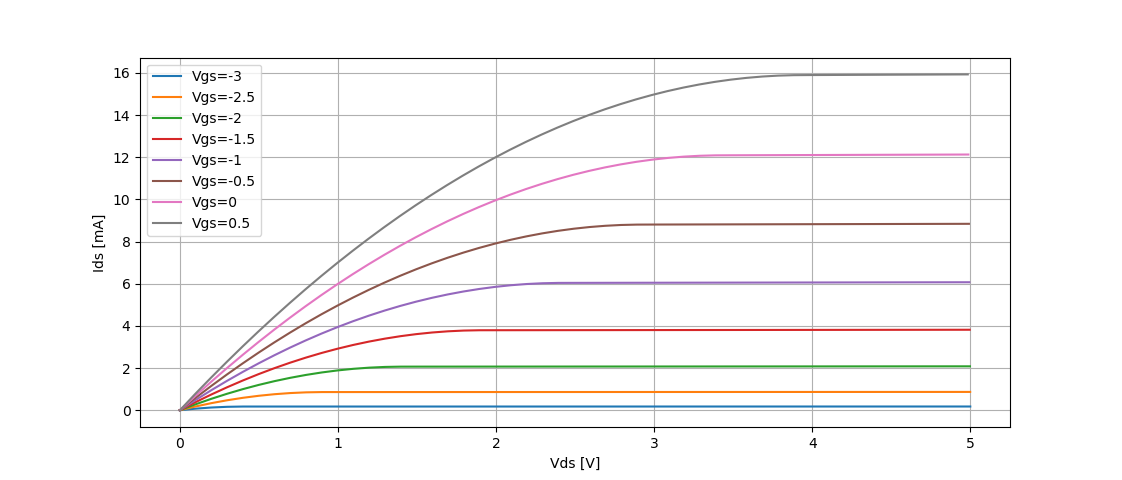
\includegraphics[width=\textwidth]{Imagenes-Ej1/curvasJfet.png}
	\label{fig:caracdcurv}
	\caption{Curvas características JFET.}
\end{figure}

\subsection{Singularidades}
Se realizaron diagramas de polos y ceros, tanto para $H(s)$ como para $T(s)$, en función de la variación de $r_d$, obteniendo los siguientes gráficos:
\begin{figure}[H]
\centering
\begin{subfigure}{.45\textwidth}
\centering
	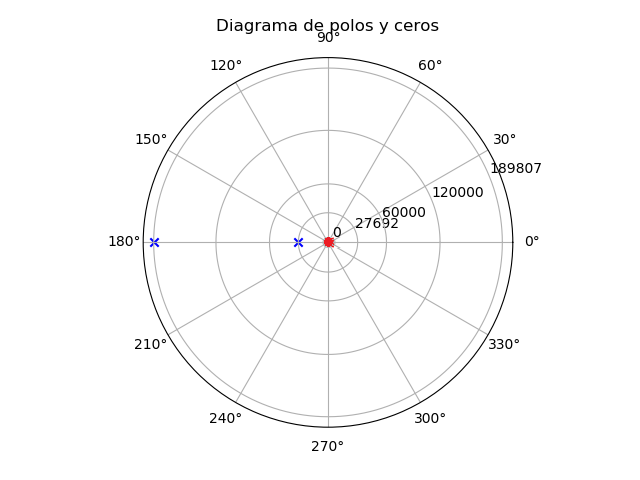
\includegraphics[width=\textwidth]{Imagenes-Ej1/Tr=1.png}
	\label{fig:poleZeroDiagTs}
	\caption{Diagrama de T(s).}
\end{subfigure}
\begin{subfigure}{.45\textwidth}
\centering
	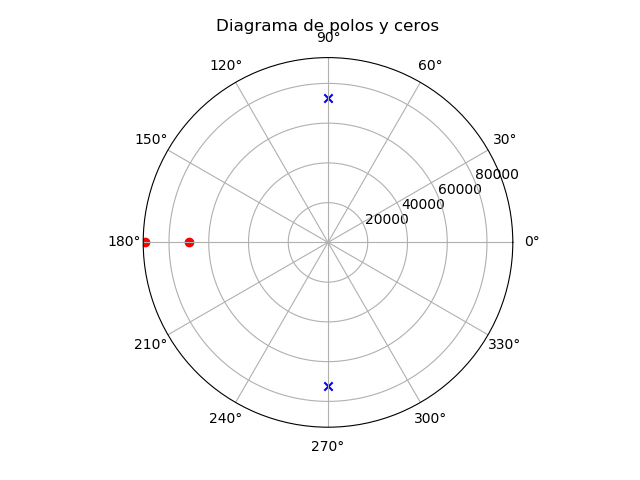
\includegraphics[width=\textwidth]{Imagenes-Ej1/Hr=1.png}
	\label{fig:poleZeroDiagHs1}
	\caption{Diagrama de H(s) con $\frac{R_2}{R_1}=2$.}
\end{subfigure}
\begin{subfigure}{.45\textwidth}
\centering
	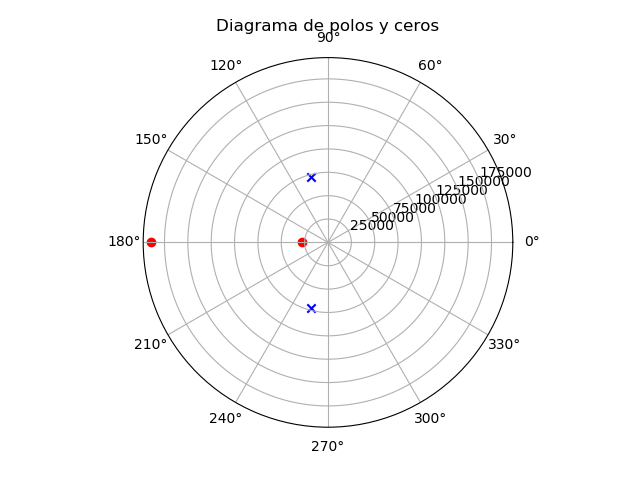
\includegraphics[width=\textwidth]{Imagenes-Ej1/Hrmin1.png}
	\label{fig:poleZeroDiagHsmin}
	\caption{Diagrama de H(s) con $\frac{R_2}{R_1}<2$.}
\end{subfigure}
\begin{subfigure}{.45\textwidth}
\centering
	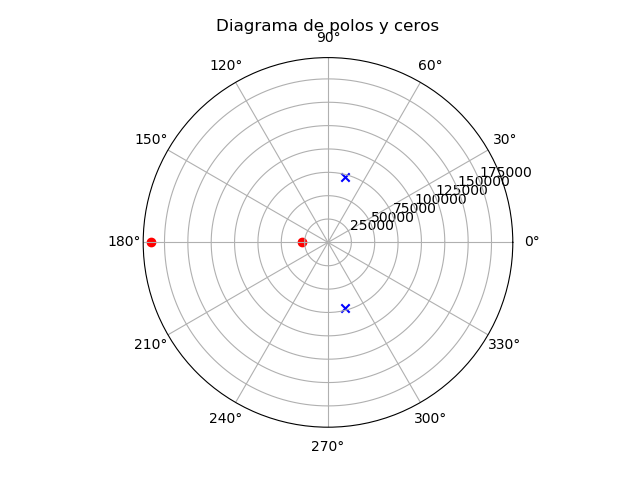
\includegraphics[width=\textwidth]{Imagenes-Ej1/Hrmn1.png}
	\label{fig:poleZeroDiagHsmax}
	\caption{Diagrama de H(s) con $\frac{R_2}{R_1}>2$.}
\end{subfigure}
\caption{Diagramas de polos y ceros.}
\label{fig:poleZeroDiag}
\end{figure}

\subsection{Elección operacional}
La exactitud y la estabilidad de la oscilación, al igual que la dinámica del amplificador operacional, resultan afectadas por la calidad de los componentes pasivos. Los capacitores y resistores SMD son buenas elecciones para los elementos en el circuito de retroalimentación positiva. En la práctica, con el fin de compensar para las tolerancias de los componentes, los circuitos de puente de Wien, con frecuencia, están equipados con correctores adecuados para el ajuste exacto de $f_o$, de aquí el uso del preset previamente mencionado sobre una de las R para ajustar dicha frecuencia.

Para evitar los efectos limitantes del slew-rate a una determinada amplitud pico de salida $V_{om}$, el amplificador operacional debe tener $SR > 2\pi V_{om} f_o$. Una vez que esta condición es cumplida, el factor limitante se convierte en el GBP finito del integrado, cuyo efecto se ve en una reducción de la frecuencia real de la oscilación. Es posible comprobar que, para mantener este cambio dentro del $10\%$ cuando se utiliza un amplificador operacional de GBP constante, este debe cumplir que $GBP \approx 43 f_o$.

El extremo inferior del rango de frecuencia depende de qué tan grandes puedan hacerse los componentes en el circuito reactivo. Con el uso de amplificadores operacionales de entrada FET para minimizar los errores de corriente de bias a la entrada, el valor de R se puede incrementar fácilmente hasta el rango de decenas de megaohms. Por ejemplo, utilizando $C = l \ \mu F$ y $R = 15.9 \ M\Omega$ se obtiene $f_o =0.01 \ Hz$.

Los amplificadores operacionales considerados son los siguientes:
\begin{table}[H]
\hspace*{-0.5cm}
\begin{tabular}{ccccccccc}
\hline
\textbf{Amplificador Operacional} & \textbf{GBP [Mhz]} & $\mathbf{SR [\frac{V}{\mu s}]}$ & $\mathbf{Z_{in} [\Omega]}$ & $\mathbf{Z_{out}[\Omega]}$ & $\mathbf{I_{bias}[A]}$ & $\mathbf{I_{off}[A]}$ & $\mathbf{V_{off}[mV]}$ & \textbf{THD} \\ \hline
\href{http://www.ti.com/lit/ds/symlink/tl082-n.pdf}{TL082}                   & 3                  & 13                              & 1T                         & -                          & 30p                 & 5p                    & 3                      & 0.003$\%$    \\
\href{http://www.ti.com/lit/ds/symlink/lm324-n.pdf}{LM324}                    & 1                  & 0.3                             & -                          & -                          & 45                  & 5                     & 2                      & -            \\
\href{http://www.ti.com/lit/ds/symlink/lm833.pdf}{LM833}                    & 10                 & 5                               & -                          & 37                         & 300n                & 10n                   & 0.3                    & 0.002$\%$    \\
\href{http://www.ti.com/lit/ds/symlink/lf356-mil.pdf}{LF356}                    & 2.5                & 12                              & 1T                         & -                          & 20p                 & 50p                   & 3                      & -            \\
\href{http://www.ti.com/lit/ds/symlink/lm741.pdf}{LM741}                    & 1.5                & 0.5                             & 2M                         & 75                         & 80n                 & 20n                   & 2                      & -            \\
\href{http://www.ti.com/lit/ds/slos070d/slos070d.pdf}{NE5534}                   & 10                 & 13                              & 100k                       & 0.3                        & 500n                & 20n                   & 0.5                    & -           \\
\hline
\end{tabular}
\caption{Comparación de operacionales.}
\end{table}

Considerando las restricciones para con el SR y GBP, las mejores opciones que se presentan son los operacionales TL082, LF356 y NE5534, donde este ultimo fue descartado debido a su baja impedancia de entrada, mientras que el LF356 debido a no contar con el dato de distorsión armónica. Finalmente queda el TL082 que es el que fue utilizado.

\subsection{Simulaciones}
Se simuló el circuito en \textbf{LTSpice} obteniendo el siguiente resultado.
\begin{figure}[H]
	\centering
	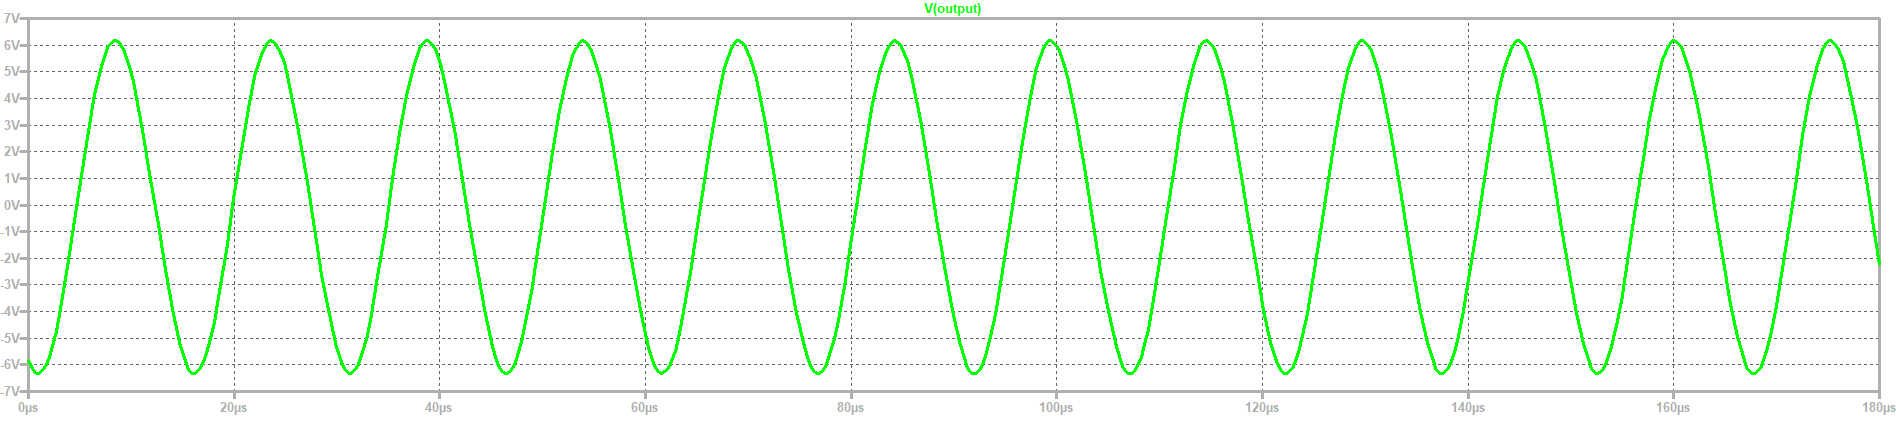
\includegraphics[width=\textwidth]{Imagenes-Ej1/osc.png}
	\caption{Simulación de la distorsión armónica.}
	\label{fig:osc}
\end{figure}

También fue posible observar el transitorio del circuito. Se puede notar como cambia la ganancia del lazo ajustándose finalmente al criterio de Barkhausen.
\begin{figure}[H]
	\centering
	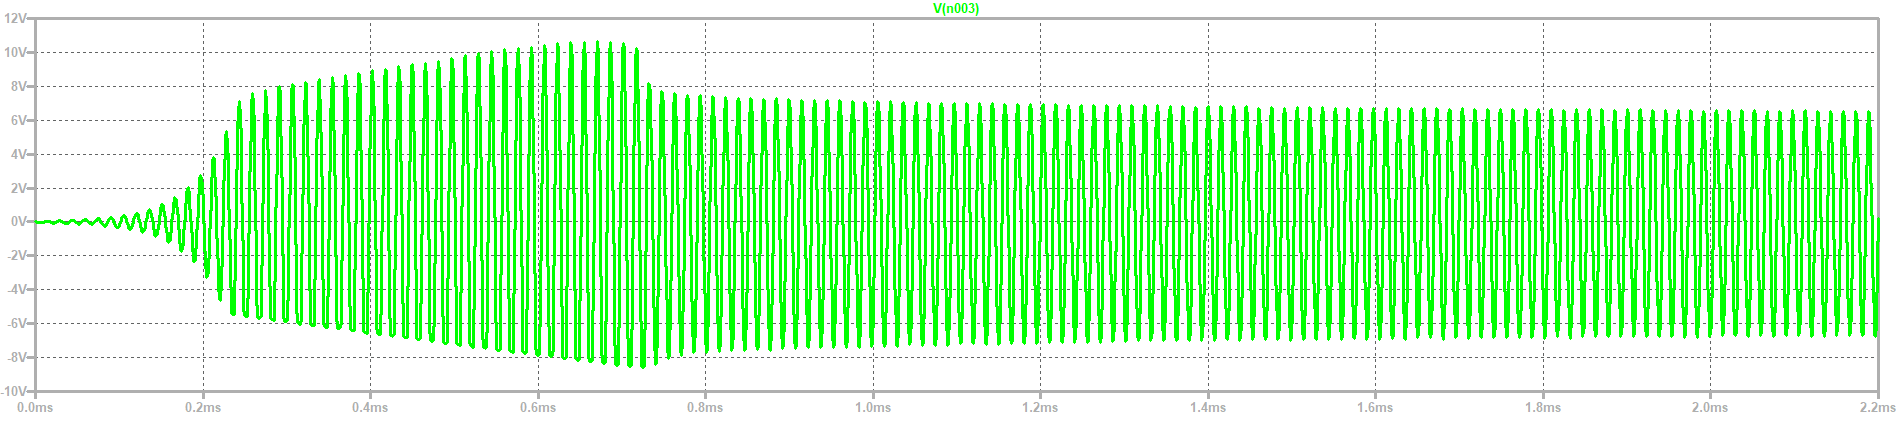
\includegraphics[width=\textwidth]{Imagenes-Ej1/trans.png}
	\caption{Respuesta transitoria.}
	\label{fig:trans}
\end{figure}

Es así que se obtuvo la distorsión armónica en la simulación Obteniendo los siguientes resultados:
\begin{table}[H]
\centering
\begin{tabular}{cccc}
\hline
\textbf{Número de armónico} & $\mathbf{Frecuencia \ [Hz]}$ & \textbf{Componente de Fourier} & \textbf{Componente Normalizada} \\
\hline
1 & $7.250 \cdot 10^{4}$ & $6.245$ & 1 \\
2 & $1.450 \cdot 10^{5}$ & $6.076 \cdot 10^{-1}$ & $9.729 \cdot 10^{-2}$ \\
3 & $2.175 \cdot 10^{5}$ & $3.477 \cdot 10^{-1}$ & $5.567 \cdot 10^{-2}$ \\
4 & $2.900 \cdot 10^{5}$ & $2.540\cdot 10^{-1}$ & $4.068 \cdot 10^{-2}$ \\
5 & $3.625 \cdot 10^{5}$ & $2.073 \cdot 10^{-1}$ & $3.319 \cdot 10^{-2}$ \\
6 & $4.350 \cdot 10^{5}$ & $1.635 \cdot 10^{-1}$ & $2.618 \cdot 10^{-2}$ \\
7 & $5.075 \cdot 10^{5}$ & $1.452 \cdot 10^{-1}$ & $2.325 \cdot 10^{-2}$ \\
8 & $5.080 \cdot 10^{5}$ & $1.308 \cdot 10^{-1}$ & $2.094 \cdot 10^{-2}$ \\
9 & $6.525 \cdot 10^{5}$ & $1.142 \cdot 10^{-1}$ & $1.828 \cdot 10^{-2}$ \\
\hline
\end{tabular}
\caption{Valores obtenidos de la simulación de distorsión armónica.}
\label{tab:distSpice}
\end{table}

\subsection{Mediciones}
Finalmente se midió el circuito realizado, obteniendo la frecuencia de oscilación deseada.
\begin{figure}[H]
	\centering
	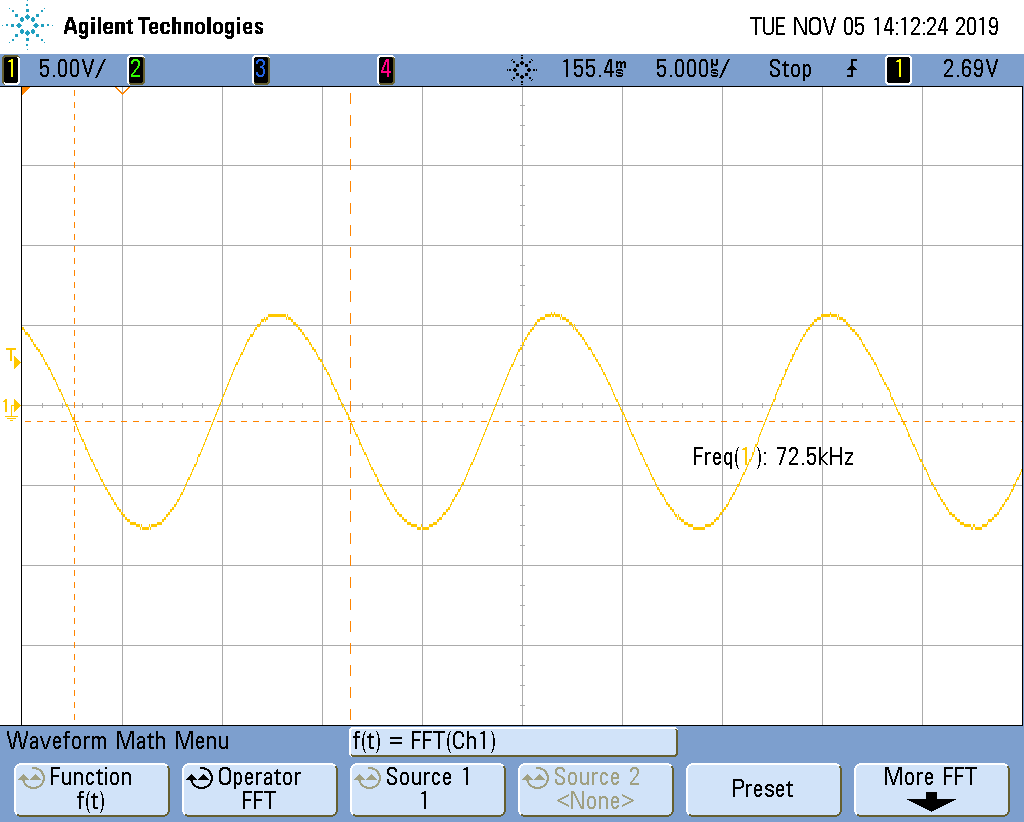
\includegraphics[width=0.5\textwidth]{Imagenes-Ej1/oscilador.png}
	\caption{Distorsión armónica medida.}
	\label{fig:trans}
\end{figure}

Aquí también se observó que el rango de valores de alimentación que puede tener el circuito varía entre $V_{max}$ del opamp y $V_p$. En en este caso se da que $V_{max}\approx 18 \ V$. También se midió el transitorio del circuito al comenzar.
\begin{figure}[H]
	\centering
	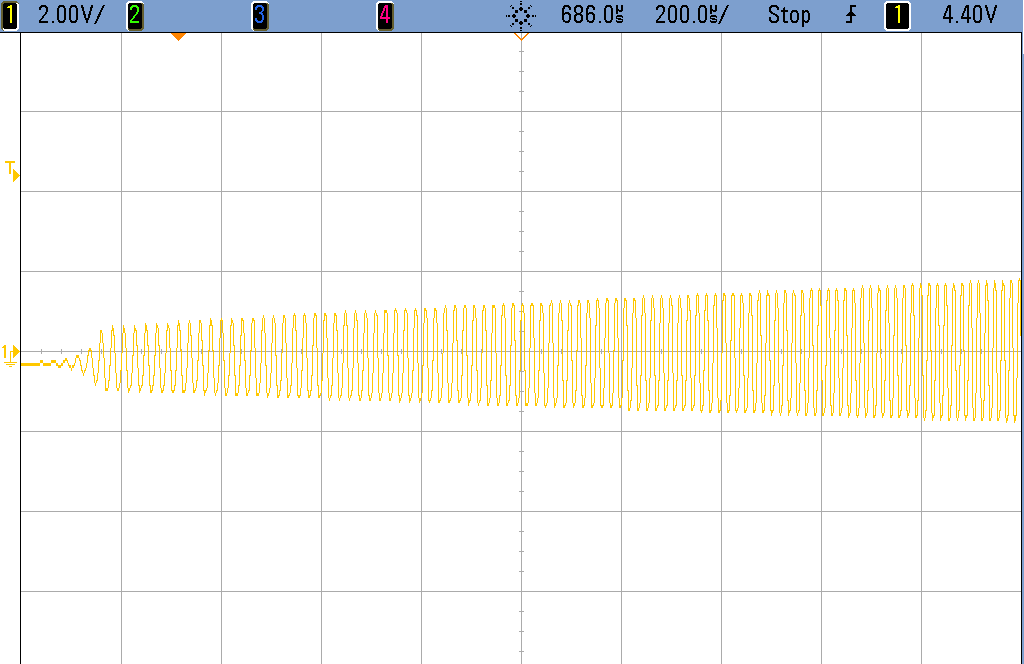
\includegraphics[width=0.5\textwidth]{Imagenes-Ej1/osciladorstep.png}
	\caption{Respuesta transitoria medida.}
	\label{fig:transStep}
\end{figure}

Es notable en la Figura (\ref{fig:transStep}) que, dado a la calibración del circuito, este posee una suave transición entre una $T(jf)>1$ hacia $T(jf) = 1$ en caso opuesto a la simulación.

También se observó que la amplitud de la señal depende de la tension de alimentación del amplificador y de la tensión de ruptura del zener. En cuanto al rango de frecuencias en las que puede trabajar, se observó que puede variar entre aproximadamente $65 \ kHz$ y $80 \ kHz$.

Además, se midió la distorsión armónica del circuito, para lo cual se valió del uso del analizador de espectros. En un principio, se observó la totalidad del espectro.
\begin{figure}[H]
	\centering
	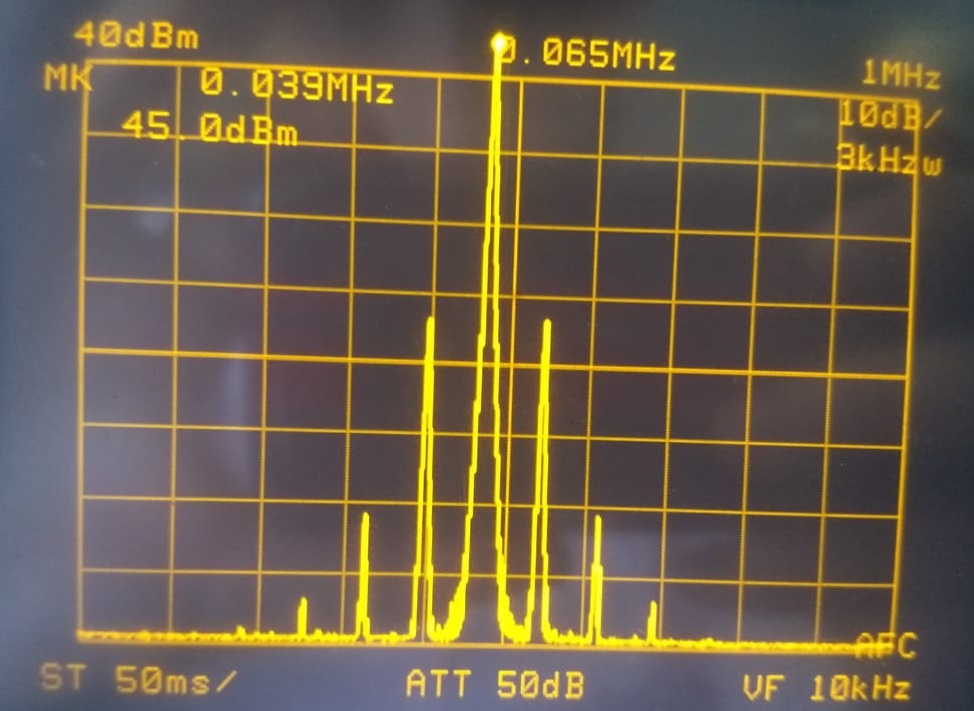
\includegraphics[width=0.5\textwidth]{Imagenes-Ej1/Espectro.jpeg}
	\caption{Espectro de la señal medido.}
	\label{fig:Espectro}
\end{figure}

Luego, se realizó una focalización en la frecuencia fundamental y en el resto de los armónicos. Es importante tener en cuenta que el analizador de espectros no se encuentra calibrado, por lo cual el 0 de la continua, que se observa como el pico central, se encuentra desplazado hacia aproximadamente $38.5 \ kHz$, por lo que los picos de la señal se encuentran desplazados.
\begin{figure}[H]
\centering
\begin{subfigure}{.4\textwidth}
\centering
	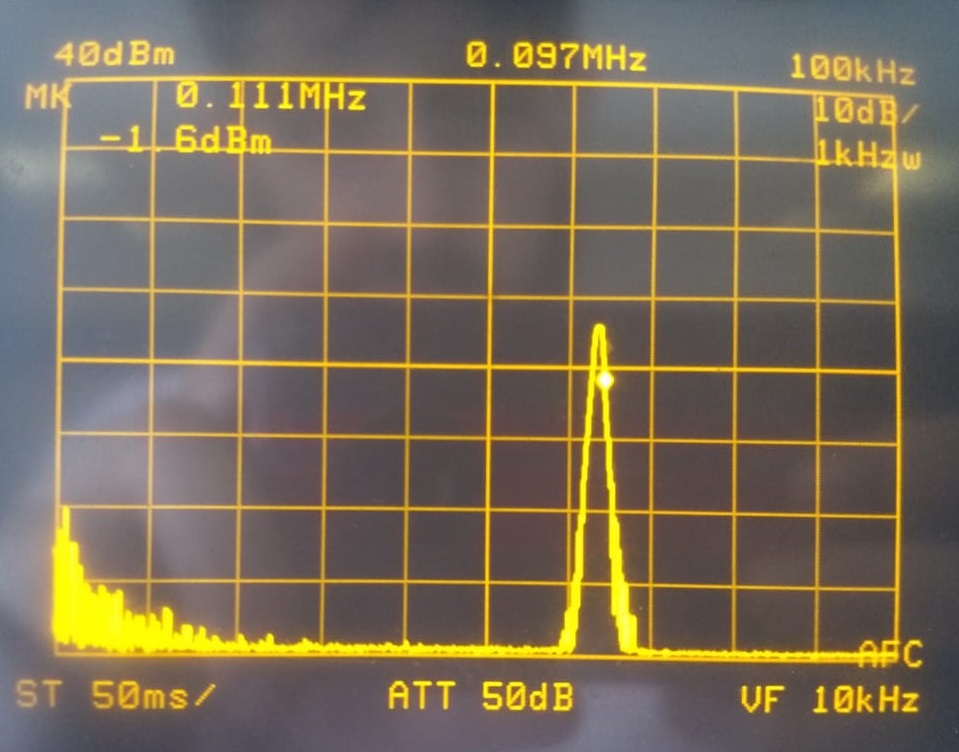
\includegraphics[width=\textwidth]{Imagenes-Ej1/Fundamental.jpeg}
	\caption{Armónico fundamental.}
	\label{fig:Fund}
\end{subfigure}
\begin{subfigure}{.425\textwidth}
\centering
	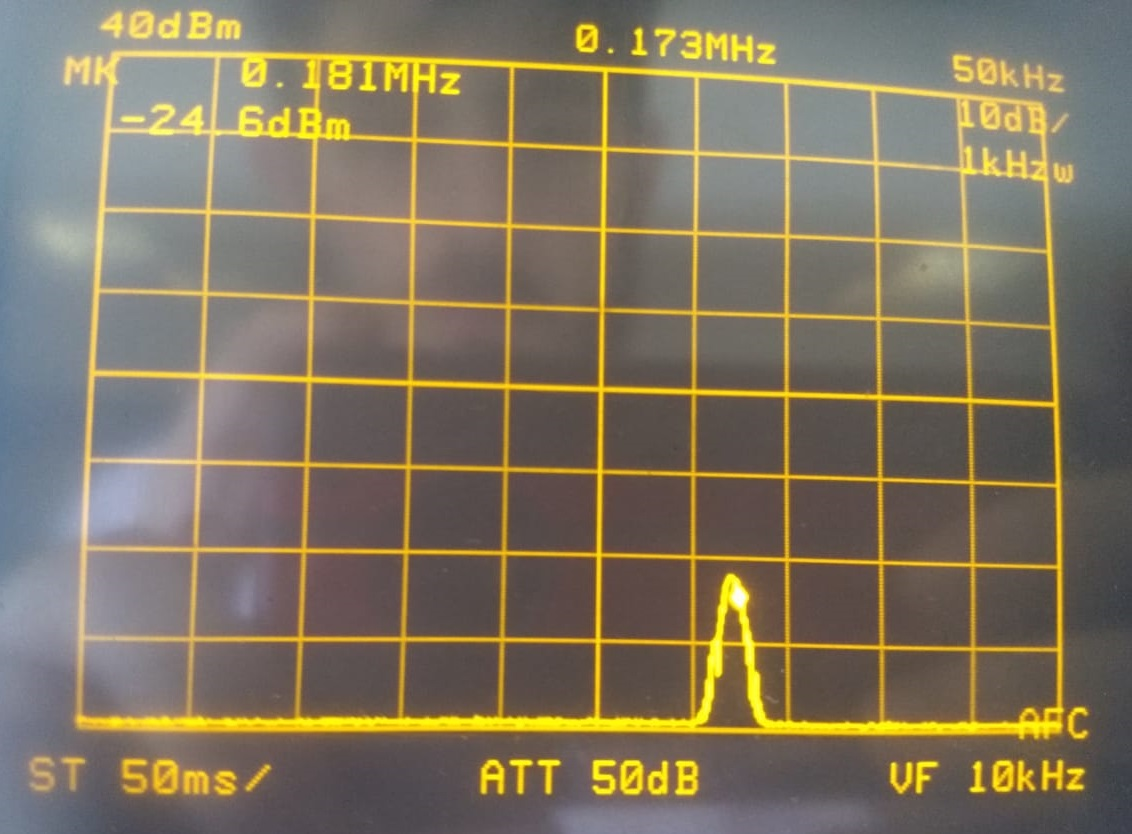
\includegraphics[width=\textwidth]{Imagenes-Ej1/1Armonico.jpeg}
	\caption{Primer armónico.}
	\label{fig:1er}
\end{subfigure}
\begin{subfigure}{.4\textwidth}
\centering
	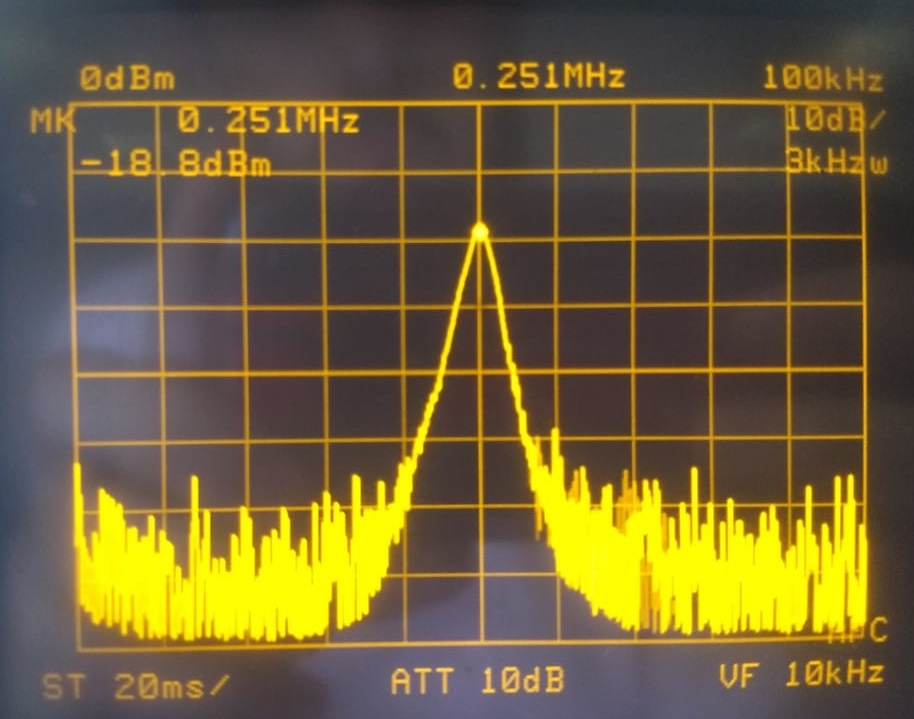
\includegraphics[width=\textwidth]{Imagenes-Ej1/2Armonico.jpeg}
	\caption{Segundo armónico.}
	\label{fig:2do}
\end{subfigure}
\begin{subfigure}{.4\textwidth}
\centering
	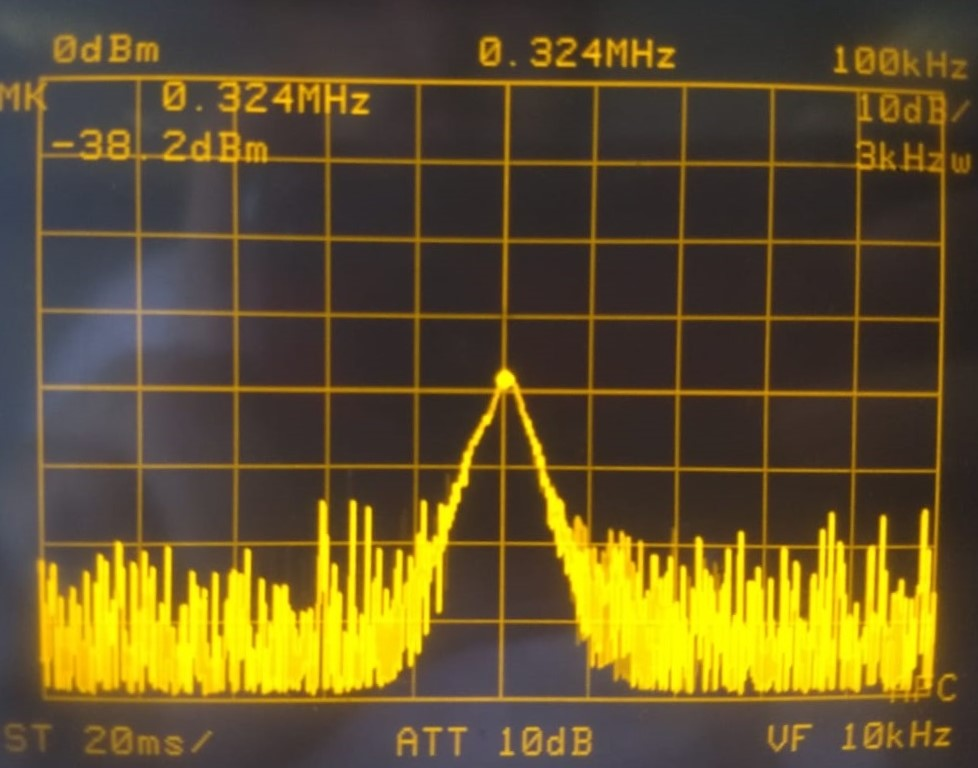
\includegraphics[width=\textwidth]{Imagenes-Ej1/3Armonico.jpeg}
	\caption{Tercer armónico.}
	\label{fig:3er}
\end{subfigure}
\begin{subfigure}{.4\textwidth}
\centering
	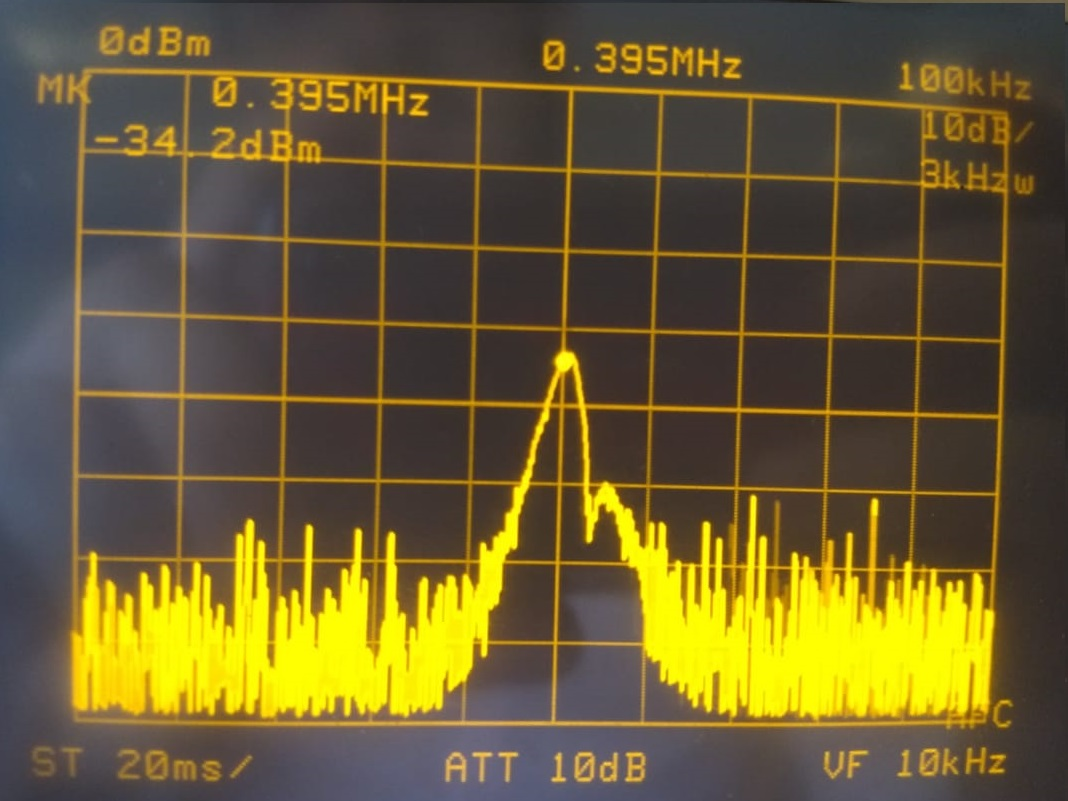
\includegraphics[width=\textwidth]{Imagenes-Ej1/4Armonico.jpeg}
	\caption{Cuarto armónico.}
	\label{fig:4to}
\end{subfigure}
\begin{subfigure}{.4\textwidth}
\centering
	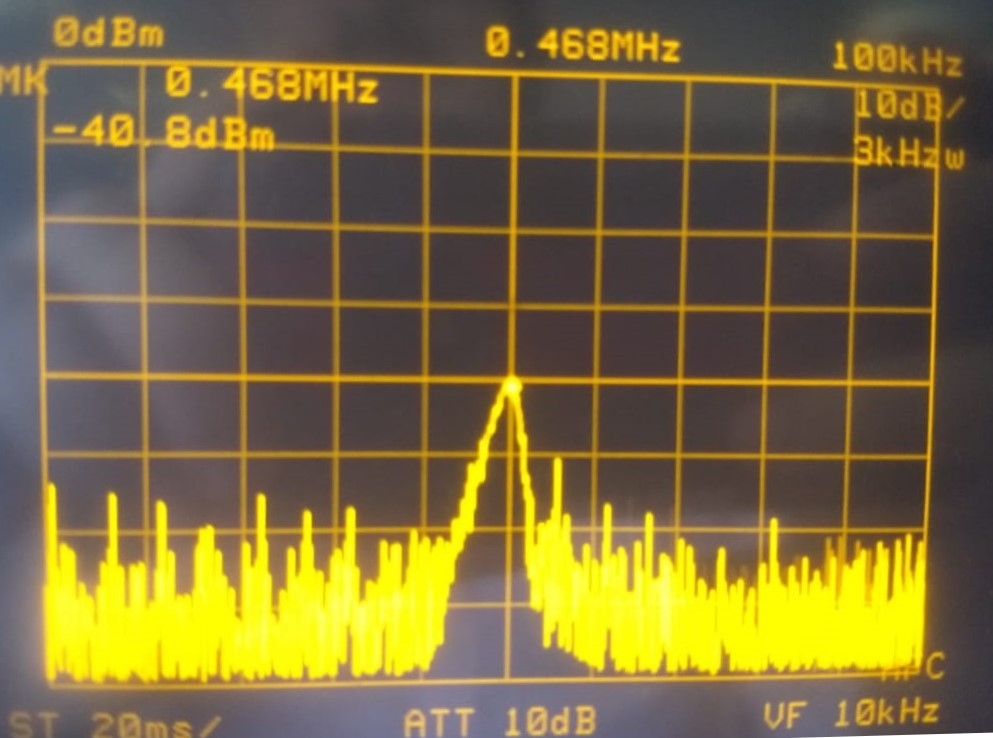
\includegraphics[width=\textwidth]{Imagenes-Ej1/5Armonico.jpeg}
	\caption{Quinto armónico.}
	\label{fig:5to}
\end{subfigure}
\begin{subfigure}{.425\textwidth}
\centering
	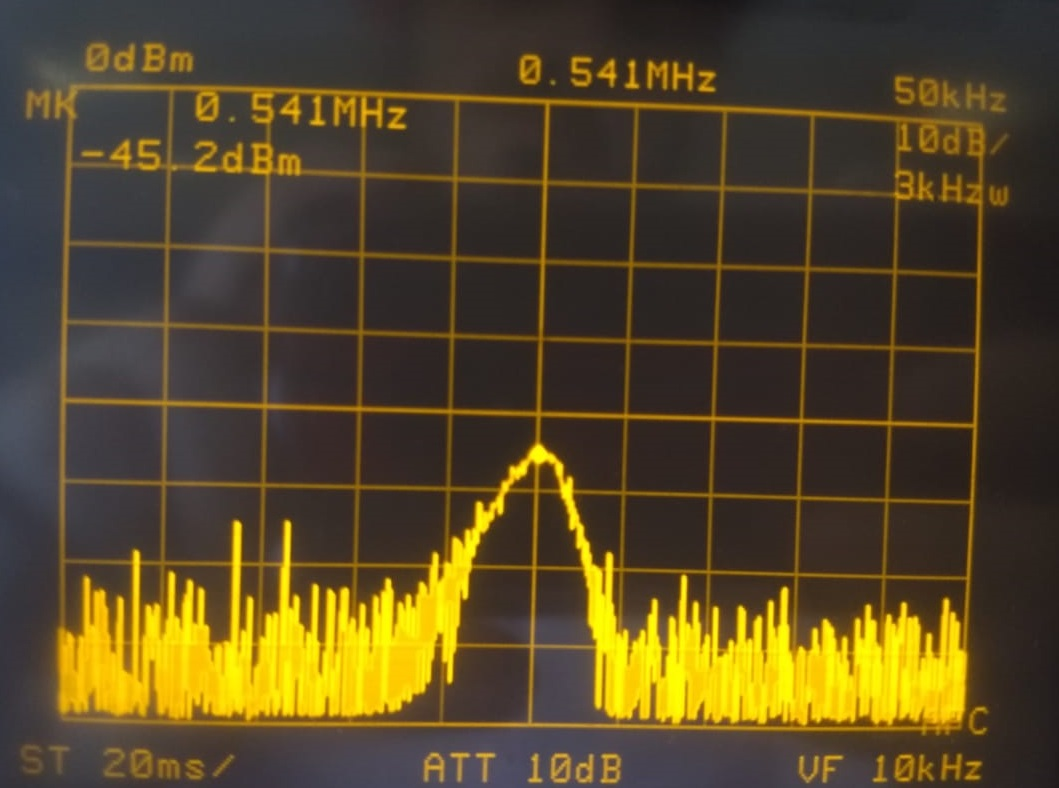
\includegraphics[width=\textwidth]{Imagenes-Ej1/6Armonico.jpeg}
	\caption{Sexto armónico.}
	\label{fig:6to}
\end{subfigure}
\caption{Armónicos medidos.}
\label{fig:armon}
\end{figure}

A partir de aquí, se puede calcular la THD bajo la siguiente fórmula:
\begin{align}
	THD= \frac{\sum_{i\neq 0} P_i}{P_0}
\end{align}

Al realizar la cuenta se obtiene un $THD \approx 0.5\%$, el cual es mucho menos al simulado. Esta gran diferencia se le atribuye a la calibración realizada en el circuito con el uso de los presets.

Luego, se midió la tensión de gate una vez alcanzado el transitorio, siendo esta de $V_g \approx -3 \ V$. Gracias a esta, la resistencia dinámica del transistor se ajuste según la tensión de salida, para permitir la oscilación.

\subsection{Conclusiones}
Se pudo realizar correctamente un oscilador de Wien, con una distorsión armónica menor al $1\%$. Este es un circuito simple, que permite generar funciones las cuales, con la introducción de un potenciómetro regulador sobre las resistencias R, puede ser convertirse en un generador de frecuencia variable, a la cual también se le puede variar al amplitud.